\section{Development}

\subsection{Flashing the Texas Instrument Sensor-Tag}
In order to flash the sensor tag, SmartRF Flash Programmer 2 made by Texas Instrument has been used. For flashing the node a sensor tag needs a Debugger DevPack, the debugger allow to communicate to the sensor via USB as it is shown in Figure \ref{fig:debug}.  
\begin{figure}[!h]
	\begin{center}
		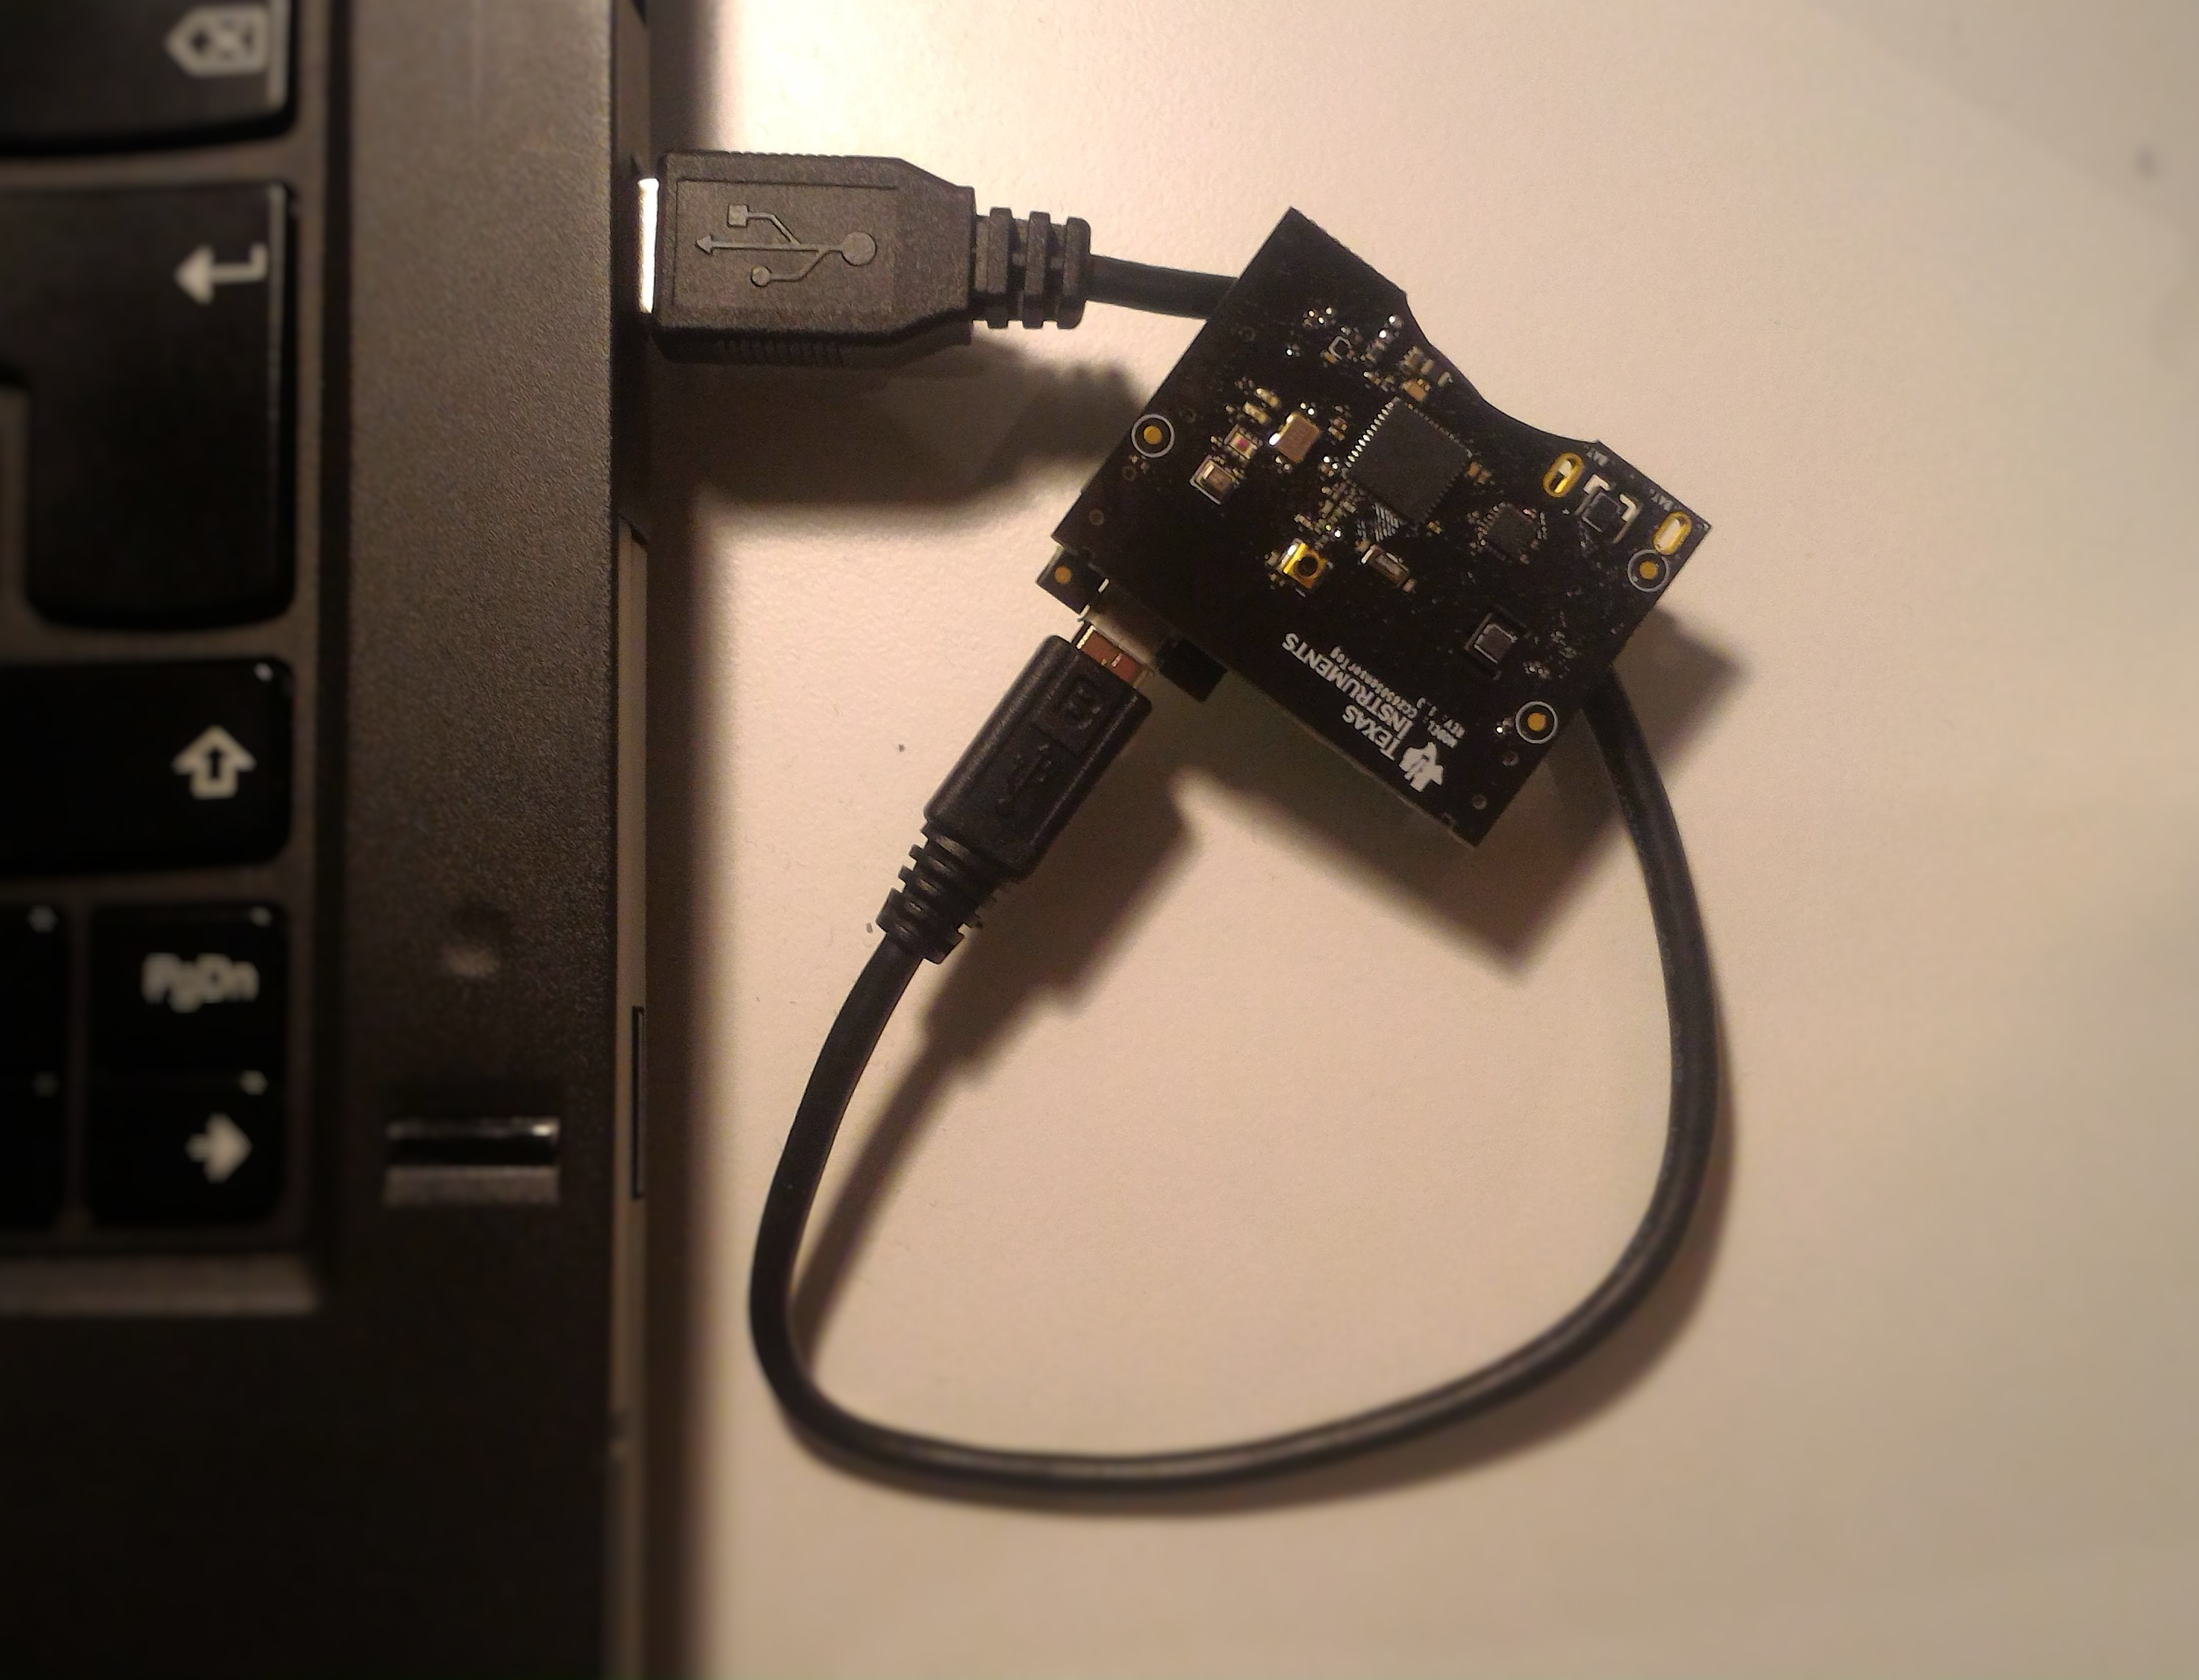
\includegraphics[width=0.8\linewidth]{debugger}
		\caption{sensor node connected with the debugger to a computer}
		\label{fig:debug}
	\end{center}
	
\end{figure} 

\subsection{title}